\begin{figure*}[htbp]
    \centering
    \vspace{1em}
    \begin{subfigure}[t]{0.32\textwidth}
        \centering
        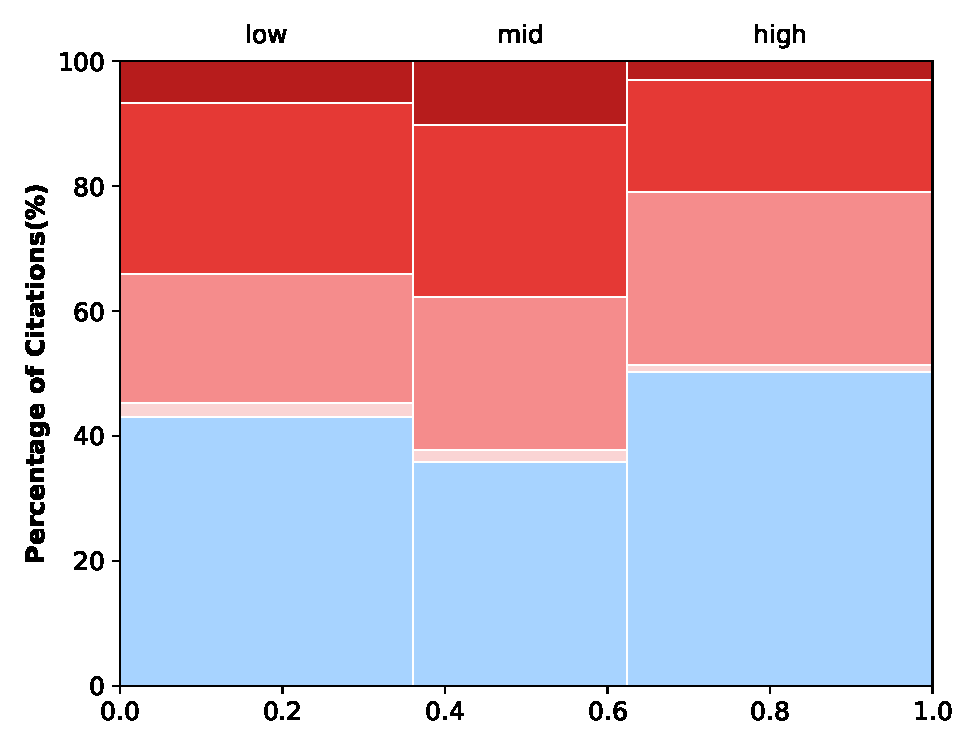
\includegraphics[width=\textwidth]{figs/coverage/citation_ratio_mekko_session-en_politics_prompts_model-openai_target-all_category-all_red_blue.pdf}
        \caption{Distributions in OpenAI (U.S.)}
        \label{fig:citation_coverage_en_openai}
    \end{subfigure}
    \begin{subfigure}[t]{0.32\textwidth}
        \centering
        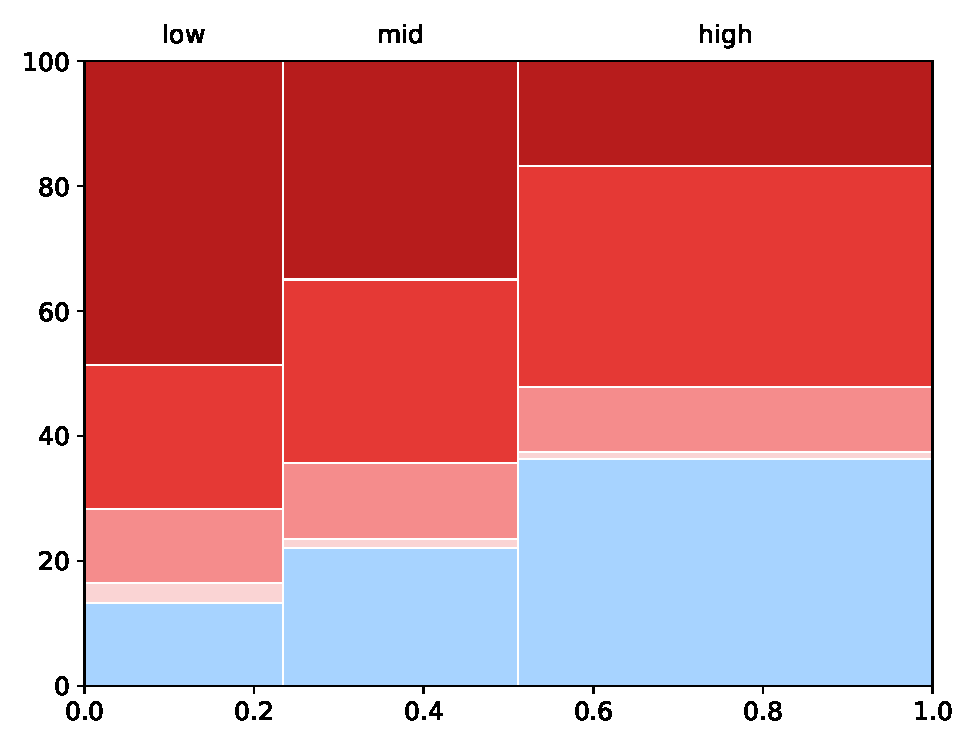
\includegraphics[width=\textwidth]{figs/coverage/citation_ratio_mekko_session-en_politics_prompts_model-gemini_target-all_category-all_red_blue.pdf}
        \caption{Distributions in Gemini (U.S.)}
        \label{fig:citation_coverage_en_gemini}
    \end{subfigure}
    \begin{subfigure}[t]{0.32\textwidth}
        \centering
        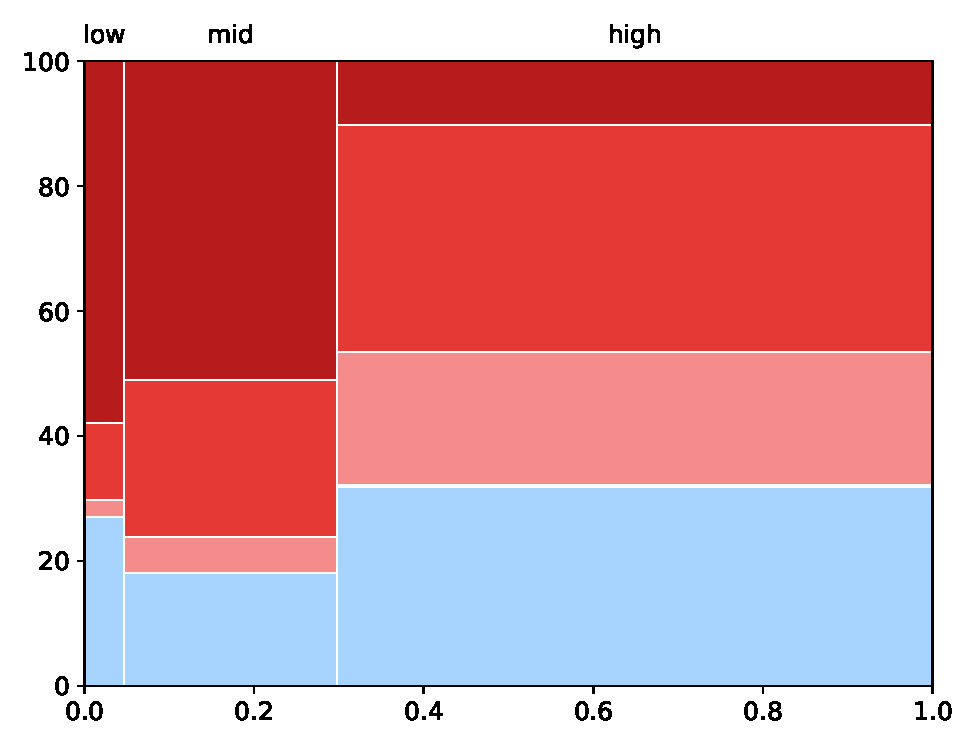
\includegraphics[width=\textwidth]{figs/coverage/citation_ratio_mekko_session-en_politics_prompts_model-claude_target-all_category-all_red_blue.pdf}
        \caption{Distributions in Claude (U.S.)}
        \label{fig:citation_coverage_en_claude}
    \end{subfigure}
    \begin{subfigure}[t]{0.32\textwidth}
        \centering
        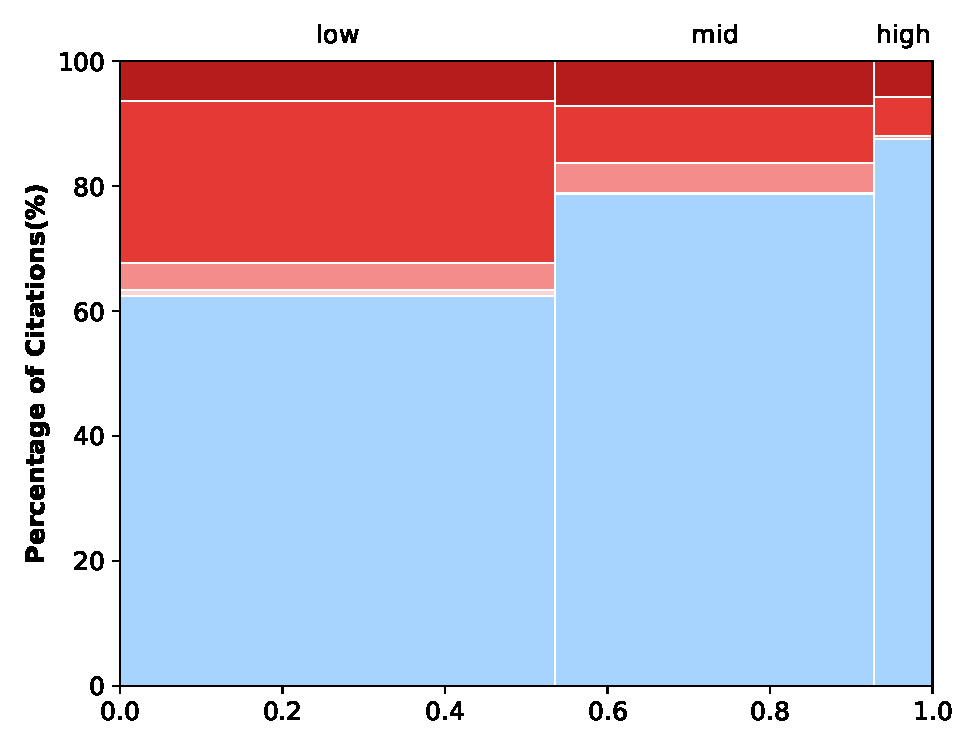
\includegraphics[width=\textwidth]{figs/coverage/citation_ratio_mekko_session-ja_politics_prompts_model-openai_target-all_category-all_red_blue.pdf}
        \caption{Distributions in OpenAI (Japan)}
        \label{fig:citation_coverage_ja_openai}
    \end{subfigure}
    \begin{subfigure}[t]{0.32\textwidth}
        \centering
        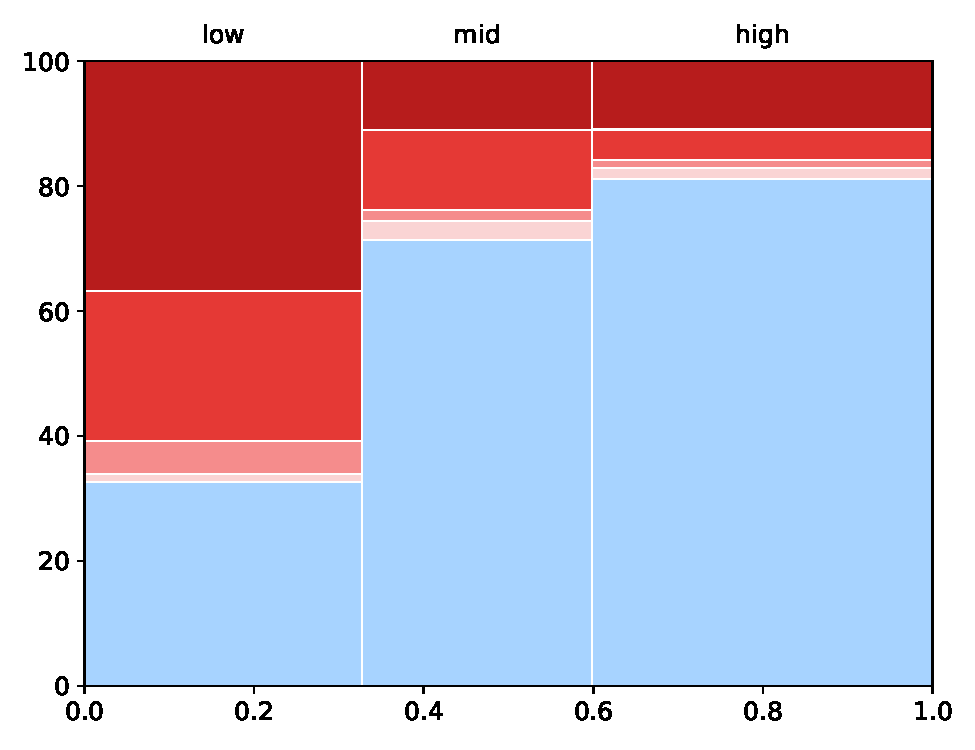
\includegraphics[width=\textwidth]{figs/coverage/citation_ratio_mekko_session-ja_politics_prompts_model-gemini_target-all_category-all_red_blue.pdf}
        \caption{Distributions in Gemini (Japan)}
        \label{fig:citation_coverage_ja_gemini}
    \end{subfigure}
    \begin{subfigure}[t]{0.32\textwidth}
        \centering
        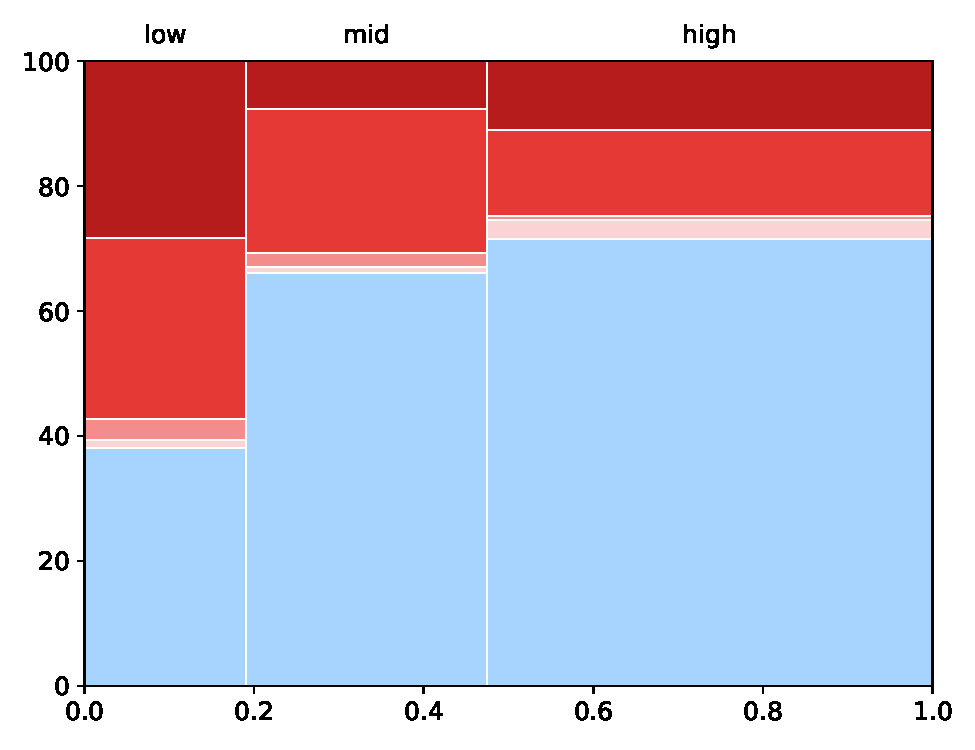
\includegraphics[width=\textwidth]{figs/coverage/citation_ratio_mekko_session-ja_politics_prompts_model-claude_target-all_category-all_red_blue.pdf}
        \caption{Distributions in Claude (Japan)}
        \label{fig:citation_coverage_ja_claude}
    \end{subfigure}
    \begin{subfigure}[t]{0.99\textwidth}
        \centering
        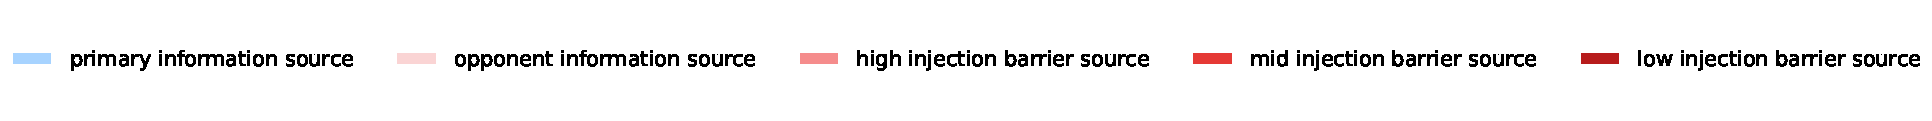
\includegraphics[width=\textwidth]{figs/full_legend.pdf}
    \end{subfigure}
    \caption{Citation coverage by similarity level for Japanese and English political prompts across models: Each chart shows the distribution of citation source types (primary, opponent, and secondary information sources categorized by attack cost) across three similarity levels(low = [-1.0, 0.8], mid = (0.8, 0.9], and high = (0.9, 1.0]).}
    \label{fig:citation_coverage}
\end{figure*}